\section{Results}

All physics, detector, environment, and baseline validation tests passed before the policy comparison. The final comparison included 30 episodes per allocation strategy.

\begin{table}[ht]
\centering
\caption{Adaptive photon-allocation performance.}
\label{tab:baseline_results}
\begin{tabular}{lccc}
\hline
Method & Detection rate & Mean photons used & Mean steps \\
\hline
Uniform & 0.767 & $1.958\times10^{12}$ & 7.83 \\
Random & 0.633 & $2.892\times10^{12}$ & 11.57 \\
Greedy & 0.900 & $1.650\times10^{12}$ & 6.60 \\
Entropy & 0.900 & $1.650\times10^{12}$ & 6.60 \\
Physics-guided information & \textbf{0.933} & $\mathbf{1.650\times10^{12}}$ & \textbf{6.60} \\
\hline
\end{tabular}
\end{table}

The physics-guided information-allocation strategy achieved the highest detection rate, reaching 93.3\%. Uniform allocation reached 76.7\%, while random allocation achieved 63.3\%.

Relative to uniform allocation, the proposed strategy improved the detection rate by approximately 21.7\% on a relative basis:

\begin{equation}
\frac{0.933-0.767}{0.767}\times100
\approx 21.7\%.
\end{equation}

Average photon consumption decreased from $1.958\times10^{12}$ photons for uniform allocation to $1.650\times10^{12}$ photons for the proposed method, corresponding to an approximate reduction of 15.7\%:

\begin{equation}
\frac{1.958-1.650}{1.958}\times100
\approx 15.7\%.
\end{equation}

The proposed method also reduced the average number of sensing actions from 7.83 to 6.60. The improvement arose from combining posterior uncertainty with the predicted optical contrast of each region. This allowed the strategy to prioritize measurements that were both uncertain and physically capable of producing informative photon returns.

Greedy and entropy allocation produced identical aggregate results in this pilot. This behavior was associated with equal initial posterior probabilities and deterministic selection under tied scores. The result should therefore be interpreted as a property of the current pilot configuration rather than evidence that the two policies are generally equivalent.

Figure~\ref{fig:detection_rate} compares the target-detection rate of the
five allocation strategies. The physics-guided information strategy achieved
the highest detection rate of 93.3\%.

\begin{figure}[ht]
\centering
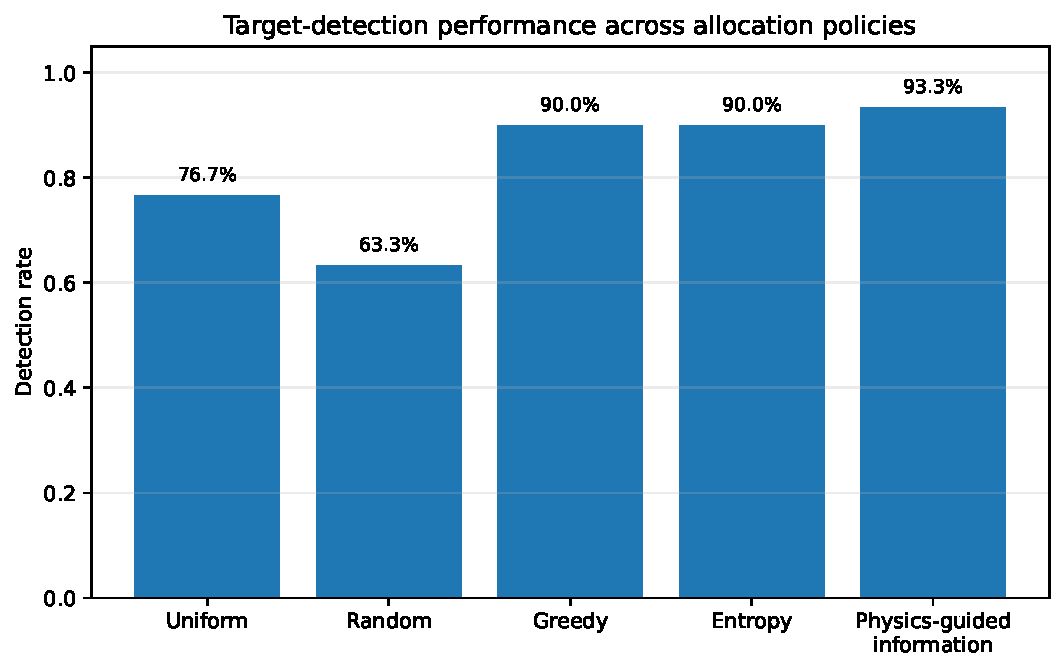
\includegraphics[width=\linewidth]{figures/final/figure_detection_rate.pdf}
\caption{Target-detection rate across the evaluated photon-allocation
strategies. Each strategy was evaluated over 30 simulated episodes.}
\label{fig:detection_rate}
\end{figure}

Figure~\ref{fig:mean_photons} compares average transmitted photon use. The
physics-guided strategy used approximately 15.7\% fewer photons than uniform
allocation.

\begin{figure}[ht]
\centering
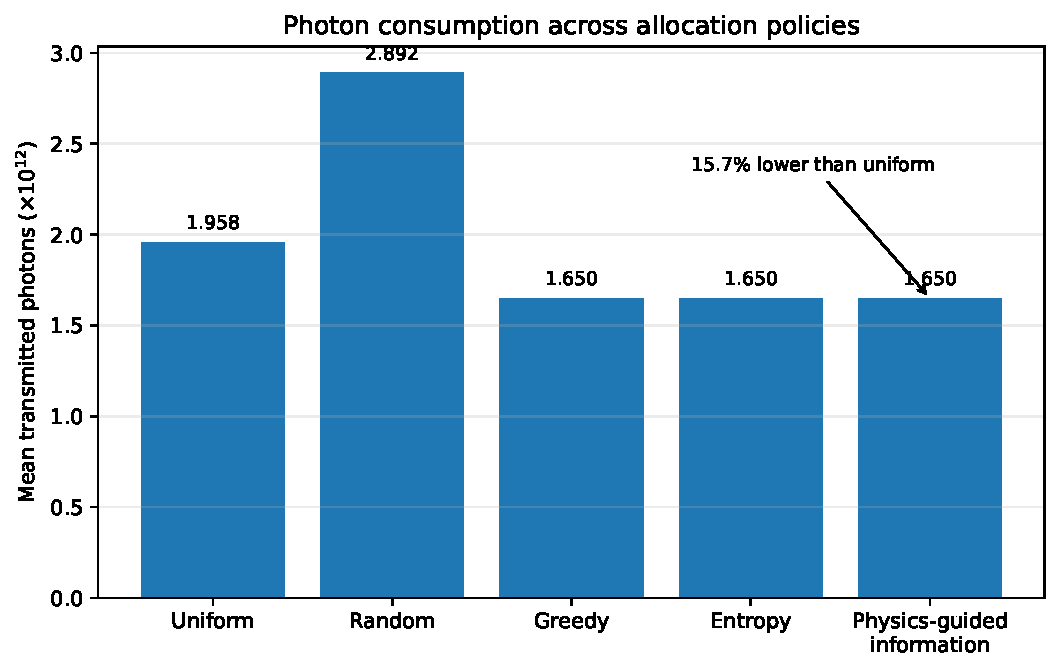
\includegraphics[width=\linewidth]{figures/final/figure_mean_photons.pdf}
\caption{Mean transmitted photon consumption across allocation strategies.
The physics-guided information strategy reduced average photon use relative
to uniform allocation.}
\label{fig:mean_photons}
\end{figure}
